\documentclass[pdftex,a4paper,twoside,11pt]{article}
\NeedsTeXFormat{LaTeX2e}

%% Include layout, additional commands and abbreviations
%%
%% Layout definitions
%%

\usepackage[english]{babel}
\usepackage[T1]{fontenc}
\usepackage[scaled=0.91]{helvet}
\usepackage{sfmath}
\usepackage{amsmath}
\usepackage{fancyhdr}
\usepackage{fancyvrb}
\usepackage[small,bf]{caption}
\usepackage{lastpage}
\usepackage{multirow}
\usepackage{tabularx}
\usepackage{longtable}
\usepackage{graphicx}
\usepackage{url}
\usepackage[usenames,dvipsnames]{color}

\definecolor{darkblue}{rgb}{0,0,0.5}
\definecolor{red}{rgb}{1,0,0}
\definecolor{green}{rgb}{0,1,0}
\definecolor{orange}{rgb}{1,0.5,0}

\usepackage[pdftex,
            colorlinks=true,
            pdfstartview=FitV,
            linkcolor=darkblue,
            citecolor=darkblue,
            urlcolor=blue,
            plainpages=false,
            pdfpagelabels,
            linktocpage,
            backref,
            pagebackref]{hyperref}

\hypersetup{
  pdftitle={METIS Reflex Tutorial},
  pdfauthor={METIS Pipeline Team},
  pdfkeywords={METIS, Data Reduction, Pipeline, Reflex, Tutorial},
  pdfsubject={METIS Reflex Tutorial}
}
\usepackage[public]{dmd-doc}

%%% Local Variables: 
%%% mode: latex
%%% TeX-master: t
%%% End:

%%
%%      UPDATE FOR NEW RELEASES
%%
\newcommand{\releasedate}{June 2022}
\newcommand{\manualversion}{1.5.0}


\newcommand{\cm}[1]{\marginpar{\scriptsize #1}}
\newcommand{\tbspa}{\rule[1ex]{0pt}{1.1ex}}
\newcommand{\tbspb}{\rule[-1.0ex]{0pt}{1.0ex}}
\newcommand{\eg}{{e.g.~}}
\newcommand{\ie}{{i.e.~}}
\newcommand{\degr}{\hbox{$^\circ$}}
\newcommand{\CPL}{\textit{Common Pipeline Library }}
\newcommand{\HDRL}{\textit{High Level Data Reduction Library }}
\newcommand{\http}[1]{\href{http://#1}{\textit{http://#1}}}


\newcommand{\putgraph}[4]{
    \subfigure
    \begin{figure}[ht]
        \begin{center}
    \includegraphics[width=#1truecm]{figures/#2}
    \end{center}
    \caption{\it #4.}
    \label{fig:#3}
    \end{figure}
}

\makeatletter
\newcommand\footnoteref[1]{\protected@xdef\@thefnmark{\ref{#1}}\@footnotemark}
\makeatother
\newcommand{\floor}[1]{\lfloor #1 \rfloor}



\dmdProgram{GEN}
\dmdProject{Science Operation Software Department}
\dmdTitle{Reflex METIS Tutorial}
\dmdDocId{ESO-XXXXXX}
\dmdDocVersion{0.4}
\dmdDocType{Manual (MAN)}
\dmdDocDate{2019-05-02}

\dmdPreparedBy{METIS Pipeline Team}
\dmdValidatedBy{}
\dmdApprovedBy{}

%% Additional commands and abbreviations
\graphicspath{{../figures/}{../pipedoc/figures/}}

%% Remember to update shortcut.tex
\def\reldate{\releasedate}
\def\pipeno{\pipelinevers}
\def\kitno{\pipeno}
\def\docno{\pipelinemanualvers}
\def\qfitsno{\qfitsvers}
\def\cplno{\cplvers}
\def\esorexno{\esorexvers}
\def\reflexno{\reflexvers}
\def\gasganono{\gasganovers}
\def\jdkno{\jdkvers}
\def\dmdissue{\docno}

\setlongtables
\makeindex
\bibliographystyle{plain} 

\begin{document}
\pagenumbering{arabic}
\dmdmaketitle
\emptypage{This page was intentionally left blank}

\section*{Authors}
\begin{tabularx}{\linewidth}{|p{0.25\linewidth}|X|}
  \hline
  \multicolumn{1}{|l|}{\textbf{Name}}\tbspa &
  \multicolumn{1}{l|}{\textbf{Affiliation}} \tbspb \\
  \hline
  \tbspa
  N.N. & Far out in the uncharted backwaters of the unfashionable end of the western spiral arm of the Galaxy
  \tbspb\\
  \hline
\end{tabularx}
\emptypage{This page was intentionally left blank}

\section*{Change Record from previous Version}
\begin{tabularx}{\linewidth}{|p{0.25\linewidth}|X|}
  \hline
  \multicolumn{1}{|l|}{\textbf{Affected Section(s)}}\tbspa &
  \multicolumn{1}{l|}{\textbf{Changes/Reason/Remarks}}\tbspb \\
  \hline
  \tbspa
  All                      & First draft
  \tbspb\\
  \hline
\end{tabularx}
\emptypage{This page was intentionally left blank}

\tableofcontents
\cleardoublepage

%\section{Introduction And Scope}
\section{Introduction to \Reflex}
This document is a tutorial designed to enable the user to to reduce
his/her data with the ESO pipeline run under an user-friendly
environmet, called {\tt EsoReflex}, concentrating on high-level issues
such as data reduction quality and signal-to-noise (S/N) optimisation.




{\tt EsoReflex} is the ESO Recipe Flexible Execution 
Workbench, an environment to run ESO VLT pipelines which employs a workflow 
engine 
% No response from kepler-project.org
%(Kepler\footnote{\http{kepler-project.org}}) 
to provide a real-time
visual representation of a data reduction cascade, called a workflow,
which can be easily understood by most astronomers. 
The basic philosophy and concepts of Reflex have been discussed by 
\href{https://ui.adsabs.harvard.edu/abs/2013A\%26A...559A..96F/abstract}{Freudling et al. (2013A\&A...559A..96F).}
Please reference this article if you use Reflex in a scientific publication.

Reflex and the data reduction workflows have been developed by ESO and 
instrument consortia and they are fully supported. If you have any issue, 
please have a look to
\href{https://support.eso.org}{https://support.eso.org} to see if this
has been reported before or 
\href{https://support.eso.org/new-ticket}{open a ticket}
for further support.


A workflow accepts science and calibration data, as downloaded from the
archive using the CalSelector
tool\footnote{\http{www.eso.org/sci/archive/calselectorInfo.html}} 
(with associated raw calibrations) and
organises them into DataSets, where each DataSet contains one
science object observation (possibly consisting of several science
files) and all associated raw and static calibrations required for a
successful data reduction. The data organisation process is fully
automatic, which is a major time-saving feature provided by the
software. The DataSets selected by the user for reduction are fed
to the workflow which executes the relevant pipeline recipes (or
stages) in the correct order.
%, providing optional user interactivity at
%key data reduction points with the aim of enabling the iteration of
%certain recipes in order to obtain better results. 
Full control of the
various recipe parameters is available within the workflow, and the
workflow deals automatically with optional recipe inputs via built-in
conditional branches. Additionally, the workflow stores the reduced
final data products in a logically organised directory structure 
employing user-configurable file names.

 %This file is in the pipedoc directory

Add here some explanation about this specific workflow. Instrument modes supported, etc...

\section{Software Installation}\label{Sec:Software_Installation}

{\tt Esoreflex} and the workflows can be installed in different ways:
via package repositories, via the\linebreak {\tt install\_esoreflex}
script or manually installing the software tar files.

 The recommended way is to use the package repositories if your
 operating system is supported. The {\tt macports} repositories
 support macOS 10.14 to 11, while the {\tt rpm/yum} repositories
 support Fedora 28 to 32, CentOS 7, Scientific Linux 7. For any other
 operating system it is recommended to use the {\tt
   install\_esoreflex} script.  

 The installation from package repository requires administrative privileges
 (typically granted via sudo), as it installs files in system-wide directories 
 under the control of the package manager. If you want a local
 installation, or you do not have sudo privileges, or if you want to
 manage different installations on different directories, then use the
 {\tt install\_esoreflex} script. Note that the script installation
 requires that your system fulfill several software prerequisites,
 which might also need sudo privileges.
 
 Reflex 2.11.x needs java JDK 11 to be installed.
 
 Please note that in case of major or minor (affecting the first two
 digit numbers) Reflex upgrades, the user should erase the
 \verb+$HOME/KeplerData+, \verb+$HOME/.kepler+ directories if present,
 to prevent possible aborts (i.e. a hard crash) of the {\tt esoreflex}
 process.

 
\subsection{Installing Reflex workflows via \texorpdfstring{{\tt macports}}{macports} }

 This method is supported for the macOS operating system. It is assumed that
 macports\linebreak (\http{www.macports.org}) is installed.
 Please read the full documentation at \newline
 \http{www.eso.org/sci/software/pipelines/installation/macports.html}.

\subsection{Installing Reflex workflows via \texorpdfstring{{\tt rpm/yum/dnf}}{rpm/yum/dnf} }

 This method is supported for Fedora 28 to 32, CentOS 7,
 Scientific Linux 7 operating systems, and requires sudo rights. To install, please follow these steps

\begin{enumerate}

\item Configure the ESO repository (This step is only necessary if the ESO repository has not already been previously configured).
  \begin{itemize}
  \item If you are running Fedora, run the following commands:
\begin{verbatim}
sudo dnf install dnf-plugins-core
sudo dnf config-manager --add-repo=ftp://ftp.eso.org/pub/dfs/
            pipelines/repositories/stable/fedora/esorepo.repo
\end{verbatim}
\item If you are running CentOS 7, run the following commands:
\begin{verbatim}
sudo yum install yum-utils ca-certificates yum-conf-repos
sudo yum install epel-release
sudo yum-config-manager --add-repo=ftp://ftp.eso.org/pub/dfs/
           pipelines/repositories/stable/centos/esorepo.repo
\end{verbatim}
\item If you are running SL 7, run the following commands:
\begin{verbatim}
sudo yum install yum-utils ca-certificates yum-conf-repos
sudo yum install yum-conf-epel
sudo yum-config-manager --add-repo=ftp://ftp.eso.org/pub/dfs/
    pipelines/repositories/stable/sl/esorepo.repo
\end{verbatim}
  \end{itemize}

\item Install the pipelines
\begin{itemize}
\item The list of available top level packages for different instruments is given by:
\begin{verbatim}
sudo dnf list esopipe-\*-all # (Fedora)
sudo yum list esopipe-\*-all # (CentOS 7, SL 7)
\end{verbatim}
 
\item To install an individual pipeline use the following (This example is for X-Shooter. Adjust the package name to the instrument you require.):
\begin{verbatim}
sudo dnf install esopipe-xshoo-all # (Fedora)
sudo yum install esopipe-xshoo-all # (CentOS 7, SL 7)
\end{verbatim}

\item To install all pipelines use:
\begin{verbatim}
sudo dnf install esopipe-\*-all # (Fedora)
sudo yum install esopipe-\*-all # (CentOS 7, SL 7)
\end{verbatim}


\end{itemize}

\end{enumerate}


 For further information, please read the full documentation at \newline
 \http{www.eso.org/sci/software/pipelines/installation/rpm.html}.
 


\subsection{Installing Reflex workflows via \texorpdfstring{{\tt install\_esoreflex}}{install\_esoreflex}}

This method is recommended for operating systems other than what
indicated above, or if the user has no sudo rights. Software
dependencies are not fulfilled by the installation script, therefore
the user has to install all the prerequisites before running the
installation script.

The software pre-requisites for {\tt Reflex \reflexvers} may be found at:\newline
  \http{www.eso.org/sci/software/pipelines/reflex\_workflows}

To install the {\tt Reflex \reflexvers} software and demo data, 
please follow these instructions:
\begin{enumerate}
  \item From any directory, download the installation script:
        {\small
        \begin{verbatim}
        wget https://ftp.eso.org/pub/dfs/reflex/install_esoreflex
        \end{verbatim}
        }

  \item Make the installation script executable:
        {\small
        \begin{verbatim}
        chmod u+x install_esoreflex
        \end{verbatim}
        }

  \item Execute the installation script:
        {\small
        \begin{verbatim}
        ./install_esoreflex
        \end{verbatim}
        }
        and the script will ask you to specify three directories: the download
        directory {\tt \verb|<|download\_dir\verb|>|}, the software
        installation directory {\tt \verb|<|install\_dir\verb|>|}, 
        and the directory to be used to store the demo data 
        {\tt \verb|<|data\_dir\verb|>|}.
        If you do not specify these directories, then the installation script 
        will create them in the current directory with default names.
        
      \item Follow all the script instructions; you will be asked
        whether to use your Internet connection (recommended: yes),
        the pipelines and demo-datasets to install (note that the
        installation will remove all previously installed pipelines
        that are found in the same installation directory).
 % \item You will be asked whether you want to use your Internet connection.
 %       Unless you want to reuse already downloaded packages (only advanced
 %       users), use the default Yes.

%  \item You will be given a choice of pipelines (with the corresponding 
 %       workflows) to install. Please specify the numbers for the pipelines 
 %       you require, separated by a space, or type ``A'' for all pipelines.

 % \item For the pipelines to be installed you will be prompted for the 
 %       demo data sets to be installed. Type ``A'' for all demo datasets.
 %       Take into account that if you are installing in a directory that 
 %       already contains data, it won't be removed.

 % \item The script will also detect whether previous versions of the 
 %       workflows or Reflex were installed and in this case you have the
 %       option to update links or remove obsolete cache directories. It is 
 %       advised to use the defaults.

 % \item If some of the prerequisite binaries for {\tt Reflex} are not under one
 %       of the paths indicated by the command,
 %       {\small
 %       \begin{verbatim}
 %       getconf PATH
 %       \end{verbatim}
 %       }
 %       then you will need to add the appropriate paths as a colon separated
 %       list to the {\tt esoreflex.path} parameter in the configuration file
 %       {\tt \verb|<|install\_dir\verb|>|/etc/esoreflex.rc}. This will usually
 %       be necessary when the FITS viewer ({\tt fv}) is installed outside of
 %       {\tt /usr/bin}. As an example, assume {\tt fv} is installed into the
 %       directory {\tt /usr/local/fv5.4}, the file {\tt esoreflex.rc} should
 %       then have the line setting {\tt esoreflex.path} look similar to the
 %       following:
 %       {\small
 %       \begin{verbatim}
 %       esoreflex.path=/usr/local/fv5.4
 %       \end{verbatim}
 %       }
 %       In the case of OS~X {\tt /Applications/fv.app/Contents/MacOS/} is the
 %       typically installation directory. Thus, this should be similar to the
 %       following line instead:
 %       {\small
 %       \begin{verbatim}
 %       esoreflex.path=/opt/local/bin:/Applications/fv.app/Contents/MacOS
 %       \end{verbatim}
 %       }
%%
  \item To start {\tt Reflex}, issue the command:
        {\small
        \begin{verbatim}
        <install_dir>/bin/esoreflex
        \end{verbatim}
        }
        It may also be desirable to set up an alias command for starting the 
        {\tt Reflex} software, using the shell command {\tt alias}. 
        Alternatively, the {\tt PATH} variable can be updated to contain the
        {\tt \verb|<|install\_dir\verb|>|/bin} directory.
\end{enumerate}

 %This file is in the pipedoc directory

\section{Demo Data}
Add some explanation about the demo data used.

\section{Quick Start: Reducing The Demo Data \label{sec:quick_start}}

Add here a two pages maximum explanation on how to quickly reduce the demo data set.

%\subsection{About the main {\tt esoreflex} canvas \label{sec:about_canvas}}
\section{About the main {\tt esoreflex} canvas \label{sec:about_canvas}}

%\subsubsection{Saving And Loading Workflows}
\subsection{Saving And Loading Workflows}

In the course of your data reductions, it is likely that you will
customise the workflow for various data sets, even if this simply
consists of editing the {\tt ROOT\_DATA\_DIR} to a different value for
each data set.  Whenever you modify a workflow in any way, you have
the option of saving the modified version to an {\tt XML} file using
{\tt File -> Export As} (which will also open a new workflow canvas
corresponding to the saved file).  The saved workflow may be opened in
subsequent {\tt esoreflex} sessions using {\tt File -> Open}. Saving the
workflow in the default Kepler format (.kar) is only advised if you do
not plan to use the workflow with another computer.

%\subsubsection{Buttons}  
\subsection{Buttons}  
         
At the top of the {\tt esoreflex} canvas are a set of buttons which have the following functions:
\begin{itemize}
\item{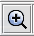
\includegraphics[width=0.5cm,height=0.5cm]{reflex_zoom_in_button.png} - Zoom in.}
\item{
\includegraphics[width=0.5cm,height=0.5cm]{reflex_zoom_reset_button.png} - Reset the zoom to 100\%.}
\item{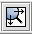
\includegraphics[width=0.5cm,height=0.5cm]{reflex_zoom_to_fit_button.png} - Zoom the workflow to fit the current window size (Recommended).}
\item{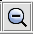
\includegraphics[width=0.5cm,height=0.5cm]{reflex_zoom_out_button.png} - Zoom out.}
\item{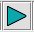
\includegraphics[width=0.5cm,height=0.5cm]{reflex_run_button.png} - Run (or resume) the workflow.}
\item{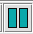
\includegraphics[width=0.5cm,height=0.5cm]{reflex_pause_button.png} - Pause the workflow execution.}
\item{
\includegraphics[width=0.5cm,height=0.5cm]{reflex_stop_button.png} - Stop the workflow execution.}
\end{itemize}
The remainder of the buttons (not shown here) are not relevant to the 
workflow execution.

%\subsubsection{Workflow States}
\subsection{Workflow States}

A workflow may only be in one of three states: executing, paused, or stopped.
 These states are indicated by the yellow highlighting of the
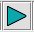
\includegraphics[width=0.5cm,height=0.5cm]{reflex_run_button.png},
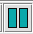
\includegraphics[width=0.5cm,height=0.5cm]{reflex_pause_button.png},
and 
\includegraphics[width=0.5cm,height=0.5cm]{reflex_stop_button.png}
buttons, respectively. A workflow is executed by clicking the
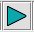
\includegraphics[width=0.5cm,height=0.5cm]{reflex_run_button.png} button. 
Subsequently the workflow and any running
pipeline recipe may be stopped immediately by clicking the

\includegraphics[width=0.5cm,height=0.5cm]{reflex_stop_button.png}
button, or the workflow may be paused by clicking the 
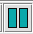
\includegraphics[width=0.5cm,height=0.5cm]{reflex_pause_button.png} button which
will allow the current actor/recipe to finish execution before the workflow is 
actually paused. 
After pausing, the workflow may be resumed by clicking the
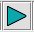
\includegraphics[width=0.5cm,height=0.5cm]{reflex_run_button.png} button again.

 %This file is in the pipedoc directory
\section{The \instname \ Workflow \label{sec:wkf_general_desc}}

The \instname\,  workflow canvas is organised into a number of areas.
From top-left to top-right you
will find general workflow instructions, directory parameters, and
global parameters.  In the middle row you will find five boxes
describing the workflow general processing steps in order from left to
right, and below this the workflow actors themselves are organised
following the workflow general steps. 

\subsection{Workflow Canvas Parameters \label{sec:wkf_canvpar}}

The workflow canvas displays a number of parameters that may be set by
the user. Under ``Setup
Directories'' the user is only required to set the {\tt
  RAW\_DATA\_DIR} to the working directory for the dataset(s) to be
reduced, which, by default, is set to the directory containing the
demo data. The {\tt RAW\_DATA\_DIR}
is recursively scanned by the {\tt Data Organiser} actor for input raw
data. The directory {\tt CALIB\_DATA\_DIR}, which is by default within the
pipeline installation directory, is also scanned by the {\tt Data
  Organiser} actor to find any static calibrations that may be missing
in your dataset(s).  If required, the user may edit the directories
{\tt BOOKKEEPING\_DIR}, {\tt LOGS\_DIR}, {\tt TMP\_PRODUCTS\_DIR}, and
{\tt END\_PRODUCTS\_DIR}, which correspond to the directories where
book-keeping files, logs, temporary products and end products are
stored, respectively (see the Reflex User Manual for further details;
\cite{REFLEXMAN}).

There is a mode of the {\tt Data Organiser} that skips the built-in
data organisation and uses instead the data organisation provided by
the CalSelector tool. To use this mode, click on {\tt Use CalSelector
  associations} in the {\tt Data Organiser} properties and make sure
that the input data directory contains the XML file downloaded with
the CalSelector archive request (note that this does not work for all
instrument workflows).

Under the ``Global Parameters'' area of the workflow canvas, the user
may set the {\tt FITS\_VIEWER} parameter to the command used for
running his/her favourite application for inspecting FITS
files. Currently this is set by default to {\tt fv}, but other
applications, such as {\tt ds9}, {\tt skycat} and {\tt gaia} for
example, may be useful for inspecting image data. Note that
it is recommended to specify the full path to the visualization
application (an alias will not work).

By default the {\tt EraseDirs} parameter is set to {\tt false}, which
means that no directories are cleaned before executing the workflow,
and the recipe actors will work in Lazy Mode (see
Section~\ref{sec:lazy_mode}), reusing the previous pipeline recipe outputs
if input files and parameters are the same as for the previous
execution, which saves considerable processing time. Sometimes it is
desirable to set the {\tt EraseDirs} parameter to {\tt true}, which
forces the workflow to recursively delete the contents of the
directories specified by {\tt BOOKKEEPING\_DIR}, {\tt LOGS\_DIR}, and
{\tt TMP\_PRODUCTS\_DIR}. This is useful for keeping disk space usage
to a minimum and will force the workflow to fully re-reduce the data
each time the workflow is run.

The parameter {\tt RecipeFailureMode} controls the behaviour in case that
a recipe fails. If set to {\tt Continue}, the workflow will trigger the next
recipes as usual, but without the output of the failing recipe, which in most
of the cases will lead to further failures of other recipes without the user
actually being aware of it. This mode might be useful for unattended processing
of large number of datasets. If set to {\tt Ask}, a pop-up window will ask
whether the workflow should stop or continue. This is the default. 
Alternatively, the {\tt Stop} mode will stop the workflow execution immediately.


\ifx\reflexinteract\undefined
\else
The parameter {\tt GlobalPlotInteractivity} controls whether the interactive
windows will appear for those windows which are {\sl enabled} by default.
The possible values are {\tt true, false}.
Take into account that some windows are disabled in the default configuration
and therefore are not affected by this parameter.
\fi

The parameter {\tt ProductExplorerMode} controls whether the {\tt
  ProductExplorer} actor will show its window or not.  The possible
values are {\tt Enabled},   {\tt Triggered}, and {\tt Disabled}.
{\tt Enabled} opens the ProductExplorer GUI at the end of the reduction of
each individual dataset. {\tt Triggered} (default and recommended) opens
the ProductExplorer GUI when all the selected datasets have been
reduced. {\tt Disabled} does not display the ProductExplorer GUI.

 %This file is in the pipedoc directory
\subsection{Workflow Actors}
\subsubsection{Simple Actors \label{sec:simple_actors}}

Simple actors have workflow symbols that consist of a single (rather
than multiple) green-blue rectangle. They may also have an icon within the rectangle
to aid in their identification. The following actors are simple actors:
\begin{itemize}
\item{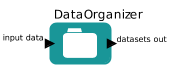
\includegraphics[width=2.5cm,height=1.3cm]{reflex_data_organiser_actor.png} - The {\tt DataOrganiser} actor.}
\item{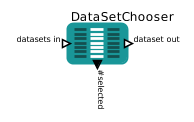
\includegraphics[width=2.5cm,height=1.6cm]{reflex_data_set_chooser_actor.png} - The {\tt DataSetChooser} actor (inside a composite actor).}
\item{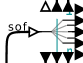
\includegraphics[width=1.6cm,height=0.8cm]{reflex_fits_router_actor.png} - The {\tt FitsRouter} actor} Redirects files according to their categories.
\item{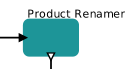
\includegraphics[width=1.8cm,height=1cm]{reflex_product_renamer_actor.png} - The {\tt ProductRenamer} actor.}
\item{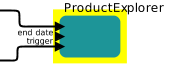
\includegraphics[width=2.2cm,height=1cm]{reflex_provenance_explorer_actor.png} - The {\tt ProductExplorer} actor (inside a composite actor).}
\end{itemize}

Access to the parameters for a simple actor is achieved by
right-clicking on the actor and selecting {\tt Configure Actor}. This
will open an ``Edit parameters'' window. Note that the {\tt Product Renamer}
actor is a jython script (Java implementation of the Python
interpreter) meant to be customised by the user (by double-clicking on
it).

 %This file is in the pipedoc directory

Add here a description of this workflow specific actors 
(probably including some composite actors).

\subsubsection{Lazy Mode \label{sec:lazy_mode}}

By default, all {\tt RecipeExecuter} actors in a pipeline workflow are
``Lazy Mode'' enabled. This means that when the workflow attempts to
execute such an actor, the actor will check whether the relevant
pipeline recipe has already been executed with the same input files
and with the same recipe parameters. If this is the case, then the
actor will not execute the pipeline recipe, and instead it will simply
broadcast the previously generated products to the output port. The
purpose of the Lazy Mode is therefore to minimise any reprocessing of
data by avoiding data re-reduction where it is not necessary.
  
One should note that the actor's Lazy Mode depends on the contents of
the directory specified by the parameter {\tt BOOKKEEPING\_DIR} and the relevant
FITS file checksums. Any modification to the directory contents and/or
the file checksums will cause the corresponding actor to run the pipeline
recipe again when executed, thereby re-reducing the input data.

The re-reduction of data at each execution may sometimes be desirable.
To force a re-reduction of data for any single {\tt RecipeExecuter} actor in
the workflow, right-click the actor, select {\tt Configure Actor}, and uncheck
the Lazy mode parameter tick-box in the ``Edit parameters'' window that is
displayed. For many workflows the {\tt RecipeExecuter} actors are actually found
inside the composite actors in the top level workflow. To access such embedded
{\tt RecipeExecuter} actors you will first need to open the sub-workflow
by right-clicking on the composite actor and then selecting {\tt Open Actor}.

To force the re-reduction of all data in a workflow (i.e. to disable
Lazy mode for the whole workflow), you must uncheck the Lazy mode for
every single {\tt RecipeExecuter} actor in the entire workflow.  It is
also possible to change the name of the bookkeeping directory, instead
of modifying any of the Lazy mode parameters. This will also force a
re-reduction of the given dataset(s). A new reduction will start (with
the lazy mode still enabled), but the results of previous reduction
will not be reused.  Alternatively, if there is no need to keep any of
the previously reduced data, one can simply set the {\tt EraseDirs}
parameter under the ``Global Parameters'' area of the workflow canvas
to {\tt true}. This will then remove all previous results that are
stored in the bookkeeping, temporary, and log directories before
processing the input data, in effect, starting a new clean data
reduction and re-processing every input dataset.  {\it Note: The
  option {\tt EraseDirs} = {\tt true} does not work in \reflex\
  version 2.9.x and makes the workflow to crash.}
 %This file is in the pipedoc directory

Add here a description of the workflow steps like Data organisation,
routing, creation of calibration files and science reduction.

Add here a description on how to optimise the results of the workflow.

\section{Frequently Asked Questions}

\begin{itemize}
   \item {\bf The error window fills the whole screen - how can I get
       to the \fbox{\tt Continue}/\fbox{\tt Stop} buttons?}

Press the \fbox{Alt} key together with your left mouse button to move
the window upwards and to the left. At the bottom the \fbox{\tt
  Continue}/\fbox{\tt Stop} buttons will be visible. This bug is known
but could not yet be fixed.

 \item {\bf I tried to {\tt Open} (or {\tt Configure}) an {\tt Actor} while the workflow is running and now it does not react any more. What should I do?}

   This is a limitation of the underlying Kepler engine. The only way
   out is to kill the workflow externally. If you want to change
   anything while a workflow is running you first need to pause it.

\item {\bf After a successful reduction of a data set, I changed this
    data set in some way (e.g. modified or removed some files, or
    changed the rules of the Data Organizer). When I restart Reflex,
    the Data Set Chooser correctly displays my new data set, but marks
    it as ``reduced ok'', even though it was never reduced before. What
    does this mean?}

  The labels in the column ``Reduced'' of the Data Set Chooser mark each
  dataset with ``OK'', ``Failed'' or ``-''. These labels indicate whether a
  data set has previously successfully been reduced at least once, all
  previous reductions failed, or a reduction has never been tried respectively.
  Data sets are identified by their name, which is derived from the first
  science file within the data set. As long as the data set name is
  preserved (i.e. the first science file in a data set has not changed),
  the Data Organizer will consider it to be the same data set. The Data
  Organizer recognizes any previous reductions of data sets it considers
  to be the same as the current one, and labels the current data set
  with ``OK'' if any of them was successful, even if the previously
  reduced data set differs from the current one.

  Note that the Product Explorer will list all the previous reductions of a
  particular data set only at the end of the reduction. This list might
  include successful and/or unsuccessful reduction runs with different
  parameters, or in your case with different input files.  The important
  fact is that these are all reductions of data sets with the same first
  raw science file. By browsing through all reductions of a particular
  raw science file, the users can choose the one they want to use.

   \item {\bf Where are my intermediate pipeline products?}
   Intermediate pipeline products are stored in the directory {\tt
   \verb|<|TMP\_PRODUCTS\_DIR\verb|>|} (defined on the workflow
 canvas, under Setup Directories)
   and organised further in directories by pipeline recipe.

%\item {\bf I have many DataSets in my data directory. How can I reduce
%  them interactively without having to wait a long time between
%  interactive windows being displayed?}

%Reduce all the DataSets at once with the interactive windows disabled
%for all interactive actors. When this reduction has finished, you
%should re-enable the interactive windows that you require, and run the
%workflow again. The workflow will run in Lazy mode and no time will be
%spent on pipeline reductions, unless you specifically change a
%parameter in one of the interactive windows.
        
%      Note that Lazy mode will not work if the workflow parameter {\tt
%        EraseDirs} is set to {\tt true}.

   \item {\bf Can I use different sets of bias frames to calibrate my
          flat frames and science data?}
   Yes. In fact this is what is currently implemented in the workflow(s).
   Each file in a DataSet has a purpose attached to it (\cite{REFLEXMAN}).
   It is this purpose that is used by the workflow to send the correct
   set of bias frames to the recipes for flat frame combination and 
   science frame reduction, which may or may not be the same set of bias 
   frames in each case.

   \item {\bf Can I run {\tt Reflex} from the command line?}
   Yes, use the command:
\begin{verbatim}
esoreflex -n <workflow_path>/<workflow>.xml
\end{verbatim}
   The -n option will set all the different options for Kepler and the
   workflows to avoid opening any GUI elements (including
   pipeline interactive windows).

   It is possible to specify workflow variables (those that appear in
   the workflow canvas) in the command line. For instance, the raw
   data directory can be set with this command:
\begin{verbatim}
esoreflex -n -RAW_DATA_DIR <raw_data_path> \
              <workflow_path>/<workflow>.xml
\end{verbatim}
   You can see all the command line options with the command 
   {\tt esoreflex -h}.

   Note that this mode is not fully supported, and the user should be 
   aware that the path to the workflow must be absolute and even if no
   GUI elements are shown, it still requires a connection to the window manager.
        
   \item {\bf How can I add new actors to an existing workflow?}
   You can drag and drop the actors in the menu on the left of the {\tt Reflex} 
   canvas. Under {\tt Eso-reflex -> Workflow} you may find all the actors
   relevant for pipeline workflows, with the exception of the recipe executer.
   This actor must be manually instantiated using
   {\tt Tools -> Instantiate Component}. Fill in the ``Class name'' field with 
   {\tt org.eso.RecipeExecuter} and in the pop-up window choose the required 
   recipe from the pull-down menu. To connect the ports of the actor, click on
   the source port, holding down the left mouse button, and release the mouse
   button over the destination port. Please consult the Reflex User Manual
   (\cite{REFLEXMAN}) for more information.

   \item {\bf How can I broadcast a result to different subsequent actors?}
   If the output port is a multi-port (filled in white), then you may have
   several relations from the port. However, if the port is a single port
   (filled in black), then you may use the black diamond from the toolbar.
   Make a relation from the output port to the diamond. Then make relations 
   from the input ports to the diamond. Please note that you cannot click to 
   start a relation from the diamond itself. Please consult the Reflex User 
   Manual (\cite{REFLEXMAN}) for more information.

   \item {\bf How can I manually run the recipes executed by Reflex?}
   If a user wants to re-run a recipe on the command line he/she has to go to
   the appropriate reflex\_book\_keeping directory, which is generally 
   reflex\_book\_keeping/<workflow>/<recipe\_name>\_<number> 
   There, subdirectories exist with 
   the time stamp of the recipe execution (e.g. 2013-01-25T12:33:53.926/). 
   If the user wants to re-execute the most recent processing he/she should 
   go to the {\tt latest} directory and then execute the script 
   {\tt cmdline.sh}. Alternatively, to use a customized {\tt esorex} command
   the user can execute
   \begin{verbatim}
   ESOREX_CONFIG="INSTALL_DIR/etc/esorex.rc"
   PATH_TO/esorex --recipe-config=<recipe>.rc <recipe> data.sof 
   \end{verbatim}
   where INSTALL\_DIR is the directory where Reflex and the pipelines were
   installed. 

   If a user wants to re-execute on the command line a recipe that used
   a specific raw frame, the way to find the proper data.sof in the bookkeeping
   directory is via {\tt grep <raw\_file> */data.sof}. 
   Afterwards the procedure is the same 
   as before.

   If a recipe is re-executed with the command explained above, the
   products will appear in the directory from which the recipe
   is called, and not in the reflex\_tmp\_products or reflex\_end\_products
   directory, and they will not be renamed. This does not happen if you use
   the {\tt cmdline.sh} script.

\ifx\reflexinteract\undefined
\else

   \item {\bf If I enter ``-'' into an empty integer parameter of an interactive
   window it is automatically completed to ``-1''. Why? }

   The parameters are validated for correctness according to their type 
   (e.g. string, integer, float). In the case of an integer or float parameter 
   ``-'' alone is considered an invalid input and is therefore automatically
   completed to ``-1''.  This is part of the validation of input done
   by the WxPython library.

\fi

\item {\bf Can I reuse the bookkeeping directory created by previous
    versions of the pipeline?}

  In general no. In principle, it could be reused if no major changes
  were made to the pipeline. However there are situations in which a
  previously created bookkeeping directory will cause problems due to
  pipeline versions incompatibility. This is especially true if the
  parameters of the pipeline recipes have changed. In that case,
  please remove the bookkeeping directory completely.

\item {\bf How to insert negative values into a textbox?}

  Due to a bug in wxPython, the GUI might appear to freeze when attempting to
  enter a negative number in a parameter's value textbox. This can be worked
  around by navigating away to a different control in the GUI with a mouse
  click, and then navigating back to the original textbox. Once focus is back
  on the original textbox the contents should be selected and it should be
  possible to replace it with a valid value, by typing it in and pressing the
  enter key.

\item {\bf I've updated my Reflex installation and when I run esoreflex the process aborts. How can I fix this problem?}
  
  As indicated in Section \ref{Sec:Software_Installation}, in case of major or
  minor (affecting the first two digit numbers) Reflex upgrades, the user
  should erase the
 \verb+$HOME/KeplerData+, \verb+$HOME/.kepler+ directories if present,
 to prevent possible aborts (i.e. a hard crash) of the esoreflex process.

\item {\bf How can include my analysis scripts and algorithms into the 
workflow?}

EsoReflex is capable of executing any user-provided script, if
properly interfaced. The most convenient way to do it is through
the Python actor. Please consult the tutorial on how to
insert Python scripts into a workflow available here:
\url{www.eso.org/sci/data-processing/Python_and_esoreflex.pdf}

\end{itemize}


Add here a section on troubleshooting problems.

%\bibliography{metis_reflex_tutorial}
\end{document}
